% !TEX root = ../my-thesis.tex
%
\chapter{Data Analysis}
\label{sec:analysis}
In this chapter the models calculated for each country are reviewed. First, a look at the standardised incidence rate for each country is taken, before spatial models, spatio-temporal models and finally regression models are discussed.
\section{Standardised Incidence Ratio}
This section takes a brief look at the standardised incidence ratio for the countries of interest.
\subsection{Standardised Incidence Ratio for Germany}
When looking at the standardised incidence ratio for Germany, it is noticeable that the actual number of infections in the eastern parts of Germany, especially in Saxony, is considerably higher than the expected number of infections. Furthermore, parts of Bavaria have an increased standardised incidence ratio compared to the rest of Germany, excluding Saxony, see Figure~\ref{sirgermany}
% \begin{figure}[H]
%   \centering
%   \includesvg[width = 1.2\textwidth]{sir_germany.svg}
%   \caption{The standardised incidence ratio for Germany based on the data of the 5th of March 2021}
%   \label{sirgermany}
% \end{figure}
\begin{figure}[H]
  \centering
  \includegraphics[width = 1.2\textwidth]{sir_germany.png}
  \caption{The standardised incidence ratio for Germany based on the data of the 5th of March 2021}
  \label{sirgermany}
\end{figure}
\subsection{Standardised Incidence Ratio for Norway}
Looking at the standardised incidence rate for Norway, a standardised incidence rate of less than 1 can be seen for most municipalities north of Trondheim. In the southern parts of Norway there are several municipalities with a rate above 1, for example the standardised incidence rate around the capital Oslo is around 2. However, the two small municipalities, Hyllestad and Ulvik, have the highest standardised incidence rate in Norway. The SIR in Hyllestad is around 5, following an outbreak in a shipyard in autumn 2020 \cite{newspaper1}, while Ulvik has a ratio of around 9, following an outbreak of the UK variant of Covid-19. According to the head of the municipality, Hans Petter Thorbjørnsen, the infections are thought to have spread through children \cite{newspaper2}. See Figure~\ref{sirnorway} for more information.
% \begin{figure}[H]
%   \centering
%   \includesvg[width = 1.2\textwidth]{sir_norge.svg}
%   \caption{The standardised incidence ratio for Norway based on the data of the 5th of March 2021}
%   \label{sirnorway}
% \end{figure}
\begin{figure}[H]
  \centering
  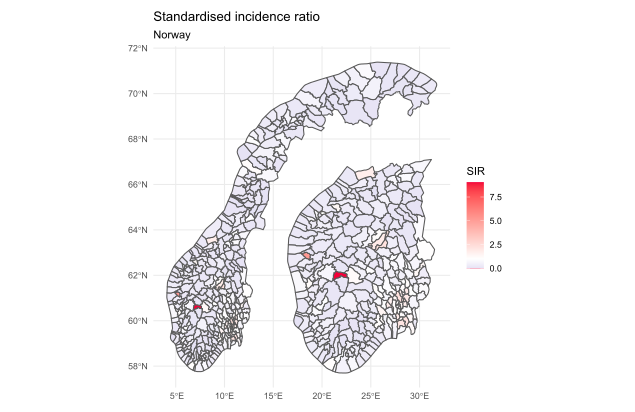
\includegraphics[width = 1.2\textwidth]{sir_norge.png}
  \caption{The standardised incidence ratio for Norway based on the data of the 5th of March 2021}
  \label{sirnorway}
\end{figure}
\clearpage
\section{Spatial Models}
After looking at the standardised incidence rates for the countries of interest, the next step is to take a closer look at the current figures for the respective countries. Spatial models are used to try to extract the factors that cause some populations to be at higher risk than other populations. Four different types of models are used for each country:
\begin{itemize}
    \item[1.] The Besarg-Yollie-Mollie Model
    \item[2.] Besags Proper Spatial Model
    \item[3.] The Leroux-Model
    \item[4.] A hierarchical model using the negative binomial distribution
\end{itemize}
Three measures are used to compare the models, the DIC, the WAIC and the CPO. \\
Before the models are computed, however, the distribution that fits the number of cases must first be found. For this, the function \texttt{descdist()} from the \texttt{fitdistrplus} R package is used. With this function, descriptive parameters of an empirical distribution can be calculated and a skewness-kurtosis plot is provided. The plots for Germany and Norway can be seen in Figure~\ref{cf_germany} and Figure~\ref{cf_norge}.
% \begin{figure}[H]
%     \centering
%     \includesvg[width = 0.8\textwidth]{cf-germany.svg}
%     \caption{The Cullen and Frey graph for Germany}
%     \label{cf_germany}
% \end{figure}
\begin{figure}[H]
    \centering
    \includegraphics[width = 0.8\textwidth]{cf-germany.png}
    \caption{The Cullen and Frey graph for Germany}
    \label{cf_germany}
\end{figure}
% \begin{figure}[H]
%     \centering
%     \includesvg[width = 0.8\textwidth]{cf_norge.svg}
%     \caption{The Cullen and Frey graph for Norway}
%     \label{cf_norge}
% \end{figure}
\begin{figure}[H]
    \centering
    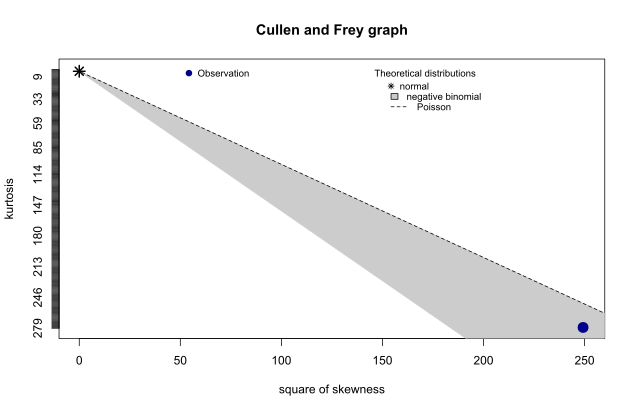
\includegraphics[width = 0.8\textwidth]{cf_norge.png}
    \caption{The Cullen and Frey graph for Norway}
    \label{cf_norge}
\end{figure}
Following these plots, a negative binomial distribution is fitted to the data using the maximum likelihood method. The function \texttt{fitdist()} is used for this. The fits can be seen in Figure~\ref{nb_germany} and Figure~\ref{nb_norge}.
% \begin{figure}[H]
%     \centering
%     \includesvg[width = 0.8\textwidth]{neg_binom_germany.svg}
%     \caption{A negative binomial fit to the number of cases in German municipalities}
%     \label{nb_germany}
% \end{figure}
\begin{figure}[H]
    \centering
    \includegraphics[width = 0.8\textwidth]{neg_binom_germany.png}
    \caption{A negative binomial fit to the number of cases in German municipalities}
    \label{nb_germany}
\end{figure}
% \begin{figure}[H]
%     \centering
%     \includesvg[width = 0.8\textwidth]{neg_binom_norge.svg}
%     \caption{A negative binomial fit to the number of cases in Norwegian municipalities}
%     \label{nb_norge}
% \end{figure}
\begin{figure}[H]
    \centering
    \includegraphics[width = 0.8\textwidth]{neg_binom_norge.png}
    \caption{A negative binomial fit to the number of cases in Norwegian municipalities}
    \label{nb_norge}
\end{figure}
Lastly, the AIC was calculated for fitting a normal distribution to the data, a Poisson distribution to the data and a negative binomial distribution to the data. The values can be seen in Table~\ref{aic}. Afterwards, the negative binomial distribution was chosen as the distribution of the target variable in both cases. \\
\begin{table}[H] 
\caption{THE AIC for different distributions for Germany and Norway \label{aic}}
\begin{tabular}{l l r}
\toprule
\textbf{Country}	& \textbf{Distribution}	& \textbf{AIC} \\
\midrule
Germany & Normal & 8364 \\
Germany & Poisson & 2065103 \\
Germany & Negative Binomial & 7726 \\
Norway & Normal & 6052 \\
Norway & Poisson & 314100 \\
Norway & Negative Binomial & 4018 \\
\bottomrule
\end{tabular}
\end{table}
For all countries, the models were computed with
\begin{itemize}
    \item[1.] only the demographic variables as covariates
    \item[2.] only the infrastructural variables as covariates
    \item[3.] both, demographic and infrastructural variables, as covariates
    \begin{itemize}
        \item[3.1] Without variable selection
        \item[3.2] With variable selection
    \end{itemize}
\end{itemize}
For each model type, different values for the penalised prior component were tried. As this resulted in a large number of models, only the model with the best performance for each model class is examined in more detail. To decide which models perform best, the DIC, WAIC and CPO are used.
\subsection{Spatial Models for Germany}
First, a look is taken at the spatial models calculated for Germany. All models are run with the INLA \cite{rinla} R package.
\subsubsection{BYM2-Models}
To specify a BYM2-2 model in R, the following code can be used:
\begin{lstlisting}[language=R]
# Specify a prior distribution
prior_1 <- list(
  prec = list(
    prior = "pc.prec",
    param = c(1, 0.01)
  )
)
# Create a neighbourhood list
nb <- poly2nb(newest_numbers_germany)
# save the neighbourhood
nb2INLA("maps/map_2.adj", nb)
# load it
g <- inla.read.graph(filename = "maps/map_2.adj")
# specify the model formula
formula_1 <- CumNumberTestedIll ~
  # add the demographic vars and pop density
  pop_dens + urb_dens + sex + 
  # specify the model with neighbourhood matrix
  f(
    idarea_1, model = "bym2", graph = g,
    scale.model = TRUE, hyper = prior_1
  ) +
  # add a random effect to the model
  f(idarea_2, model = "iid")
# compute the model
res_1 <- inla(
  formula_1,
  family = "nbinomial",
  data = newest_numbers,
  E = expected_count,
  control.predictor = list(
    compute = TRUE
  ),
  control.compute = list(dic = TRUE, waic = TRUE, cpo = TRUE)
)
\end{lstlisting}
In the example above, a random effect is added to the model. As this random effect can sometimes cover the true effects, models with and without such an effect were computed. \\
\textbf{Models Based on the Demographic Variables} \\
The best performing model based on demographic variables used the following formula and achieved the following performance:
\begin{lstlisting}[language=R]
prior_2 <- list(
  prec = list(
    prior = "pc.prec",
    param = c(0.5 / 0.31, 0.01)
  )
)
formula_10 <- CumNumberTestedIll ~
  pop_dens + urb_dens + sex + trade_tax + income_total +
  f(
    idarea_1, model = "bym2", graph = g,
    scale.model = TRUE, hyper = prior_2
  )
\end{lstlisting}
\begin{table}[H] 
\caption{The performance measures for model 10 \label{model10}}
\begin{tabular}{l l r}
\toprule
\textbf{Model}	& \textbf{Performance Measure}	& \textbf{Value} \\
\midrule
Model 10 & DIC & 5627 \\
Model 10 & WAIC & 5557 \\
Model 10 & CPO & -3366 \\
\bottomrule
\end{tabular}
\end{table}
The fixed effects summaries are presented in Table~\ref{fixed10}. It can be seen that higher population density, higher urban density and more trade tax revenue, as well as more income in general, result in a population having a higher risk of contracting Covid-19. The risk of becoming infected decreases when the proportion of women in a population increases.
\begin{table}[H] 
\caption{The fixed effects for model 10. Values are rounded. \label{fixed10}}
\begin{tabular}{l r r r r}
\toprule
\textbf{Variable}	& \textbf{Mean}	& \textbf{SD} \\
\midrule
(Intercept) & 1.61 & 1.07 \\
pop\_dens & 0.000051 & 0.000026 \\
urb\_dens & 0.053 & 0.058 \\
sex & -3.43 & 2.12 \\
trade\_tax & 0.00000000023 & 0.00000000042 \\
income\_total &  0.0000000012 & 0.0000000042 \\
\bottomrule
\end{tabular}
\end{table}
\textbf{Models Based on the Infrastructure Variables} \\
\textbf{Models Based on All Variables} \\
\textbf{Models Based on Variable Selection} 
\subsubsection{Besag-Proper-Models}
\subsubsection{Leroux-Models}
\subsubsection{Hierarchical Models}
\subsection{Spatial Models for Norway}
\clearpage
\section{Spatio-Temporal Models}
\subsection{Spatio-Temporal Models for Germany}
\subsection{Spatio-Temporal Models for Norway}
\section{Regression Models}
\clearpage
\subsection{Regression Models for Germany}
\subsection{Regression Models for Norway}